\section{Drift Robustness: Supplementary Details}
\label{sec:appendix-dedrift}

This section provides cross-configuration validation of the drift robustness conclusions established in \S\ref{sec:eval-dedrift}. The main text demonstrated that de-drifted energy remains stable across both the sizing and gating dimensions under varying drift conditions, based on a single set of probe parameters. Here, we extend that validation to a broader range of probe parameters and fault pressures, and additionally verify that triage accuracy is unaffected by the choice of statistic, justifying the use of de-drifted energy throughout the pipeline.

Table~\ref{tab:c2-1} summarizes the full experimental setup. The base configuration corresponds to the primary experiment in \S\ref{sec:eval-dedrift}; two extended configurations are used for cross-configuration validation. The three score types correspond to the statistics evaluated in the experiments: \texttt{dedrift\_countscore} is the de-drifted energy $E_s$ defined in the main text, while \texttt{raw\_sq\_sum} (raw second moment) and \texttt{abs\_net\_sum} (absolute first moment) serve as negative controls. These three statistics are evaluated on the full cross-product grid of drift intensity, workload, and probe parameters.

\begin{table}[!htbp]
\centering
\small
\setlength{\tabcolsep}{3pt}
\begin{tabular}{@{}lp{0.74\columnwidth}@{}}
\toprule
Parameter & Values \\
\midrule
Score type & \shortstack[l]{\texttt{dedrift\_countscore} (primary),\\ \texttt{raw\_sq\_sum} (negative control),  \\ \texttt{abs\_net\_sum} (negative control)} \\
$q$ & $\{0.2, 0.5, 0.9\}$ \\
Workload & $\{\text{bimodal},\ \text{heavy\_share},\ \text{diffuse}\}$ \\
\midrule
Base config & $L=4096,\ m_0=16,\ W=4,\ V=2,\ k=3,\ B=10$ \\
Extended ($V/W$) & $V \in \{2,3\},\ W \in \{2,4\},\ B=10$ \\
Extended (high $B$) & $V \in \{2,3\},\ W \in \{2,4\},\ B \in \{100, 500\}$ \\
\bottomrule
\end{tabular}
\caption{Experimental setup for drift robustness evaluation (full cross-product grid, 30 repetitions per point).}
\label{tab:c2-1}
\end{table}

\subsection{Cross-Configuration Stability of Sizing}

\begin{table*}[!thbp]
\centering
\small
\setlength{\tabcolsep}{4pt}
\begin{tabular}{@{}lclrrp{0.30\textwidth}@{}}
\toprule
\texttt{score\_type} & \texttt{q} & Workload & \texttt{median(rel\_err)} & \texttt{p90(rel\_err)} & Interpretation \\
\midrule
\texttt{raw\_sq\_sum} & 0.2 & bimodal & +16659.2\% & +17418.0\% & Orders-of-magnitude bias (failure) \\
\texttt{raw\_sq\_sum} & 0.9 & bimodal & +29576.3\% & +31180.0\% & Orders-of-magnitude bias (failure) \\
\texttt{raw\_sq\_sum} & 0.5 & bimodal & +0.4\% & +5.4\% & Normal \\
\texttt{raw\_sq\_sum} & 0.9 & diffuse & +132.5\% & +134.3\% & Significant bias \\
\texttt{dedrift\_countscore} & 0.2 & bimodal & -9.1\% & -4.1\% & Normal \\
\texttt{dedrift\_countscore} & 0.5 & bimodal & -9.1\% & -5.0\% & Normal \\
\texttt{dedrift\_countscore} & 0.9 & bimodal & -8.9\% & -3.7\% & Normal \\
\texttt{dedrift\_countscore} & 0.5 & diffuse & -9.3\% & -8.9\% & Normal \\
\texttt{dedrift\_countscore} & 0.5 & heavy\_share & -9.2\% & -6.6\% & Normal \\
\texttt{abs\_net\_sum} & 0.5 & bimodal & -95.0\% & -94.9\% & Significant bias \\
\bottomrule
\end{tabular}
\caption{Representative numerical values from Table~\ref{tab:c2-unified}: sizing error under drift for different score types.}
\label{tab:c2-2}
\end{table*}

Table~\ref{tab:c2-2} expands selected rows from the main-text Table~\ref{tab:c2-unified} with additional workloads. Because the full cross-product grid is too large to present in tabular form, Figure~\ref{fig:c2-a2} summarizes the extended high-$B$ settings ($B \in \{100, 500\}$) compactly, plotting \texttt{p90(|rel\_err|)} rather than signed error. The same separation pattern persists throughout the full grid: de-drifted energy remains stable and nearly invariant to drift; the raw second moment still exhibits failures on the order of $10^4\%$ under strong drift; and the first moment consistently falls in the $20\%$--$96\%$ range. The $V/W$ parameter sweep yields the same conclusion and is omitted for brevity.

\begin{figure*}[!thbp]
\centering
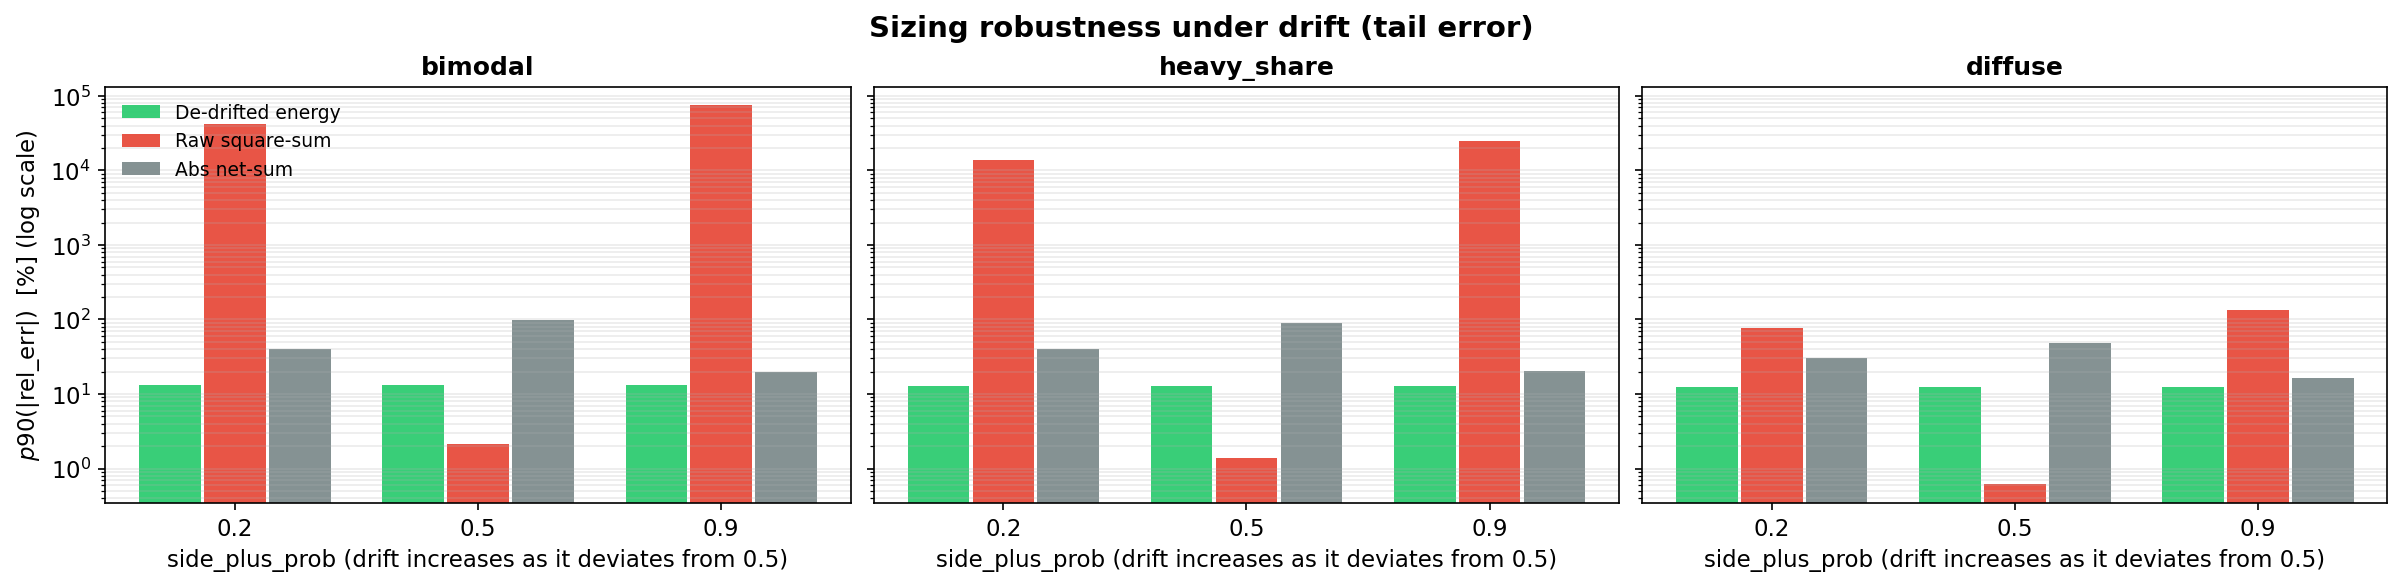
\includegraphics[width=0.9\textwidth]{figures/fig_exp03v2_sizing_p90_abs_relerr_vs_drift.png}
\caption{Drift robustness of sizing under extended configurations ($B \in \{100, 500\}$, $V \in \{2,3\}$, $W \in \{2,4\}$). The figure plots \texttt{p90(|rel\_err|)} to compare error magnitude. The de-drifted statistic remains stable across the full drift range. Y-axis is on a log scale.}
\label{fig:c2-a2}
\end{figure*}


\begin{table}[!thbp]
\centering
\footnotesize
\setlength{\tabcolsep}{3pt}
\begin{tabular}{@{}p{0.34\linewidth}ccc@{}}
\toprule
Metric & \shortstack[c]{Base config\\(\S\ref{sec:eval-dedrift})} & \shortstack[c]{Extended\\($V/W$)} & \shortstack[c]{Extended $B$\\($\{100,500\}$)} \\
\midrule
\makecell[l]{\texttt{median(rel\_err)}\\(across drift range)} & [-9.25, -9.17] & [-10.41, -10.28] & [-10.65, -10.46] \\
\cmidrule(lr){1-4}
\makecell[l]{\texttt{median(rel\_err\_scaled)}\\(across drift range)} & [-3.19, -3.12] & [-4.44, -4.30] & [-4.69, -4.49] \\
\cmidrule(lr){1-4}
\makecell[l]{Convergence\\magnitude (pp)} & $\approx$ +6.06 & $\approx$ +5.98 & $\approx$ +5.96 \\
\bottomrule
\end{tabular}
\caption{Sizing bias before and after Bessel correction (units: \%). }
\label{tab:c2-3}
\end{table}

After applying the Bessel-type scaling $\hat{D}^{\text{scaled}} = \hat{D} \cdot m_0/(m_0{-}1)$, the systematic underestimation converges from approximately $-9\%$ to approximately $-3\%$. Table~\ref{tab:c2-3} summarizes the numerical ranges across the base configuration and two extended sweeps: the convergence magnitude remains at approximately 6 percentage points across all configurations, indicating that this correction effect is governed by the structural properties of the statistic.


\subsection{Cross-Configuration Stability of Gating}

\begin{table}[!htbp]
\centering
\small
\begin{tabular}{llccc}
\toprule
$B$ & Score type & $q{=}0.2$ & $q{=}0.5$ & $q{=}0.9$ \\
\midrule
\multirow{2}{*}{10} & \texttt{dedrift\_countscore} & 0.0153 & 0.0166 & 0.0162 \\
                    & \texttt{abs\_net\_sum}       & 0.0198 & \textbf{0.425} & 0.0187 \\
\midrule
\multirow{2}{*}{500} & \texttt{dedrift\_countscore} & 0.430 & 0.426 & 0.428 \\
                     & \texttt{abs\_net\_sum}        & 0.490 & \textbf{0.745} & 0.411 \\
\bottomrule
\end{tabular}
\caption{$K_{\mathrm{eff}}/L$ for two statistics under \texttt{heavy\_share} ($B{=}10$ and $B{=}500$). De-drifted energy remains stable across both $B$ levels and all three drift conditions; the first moment exhibits anomalous inflation at $q{=}0.5$.}
\label{tab:c2-5}
\end{table}


\begin{figure*}[!thbp]
\centering
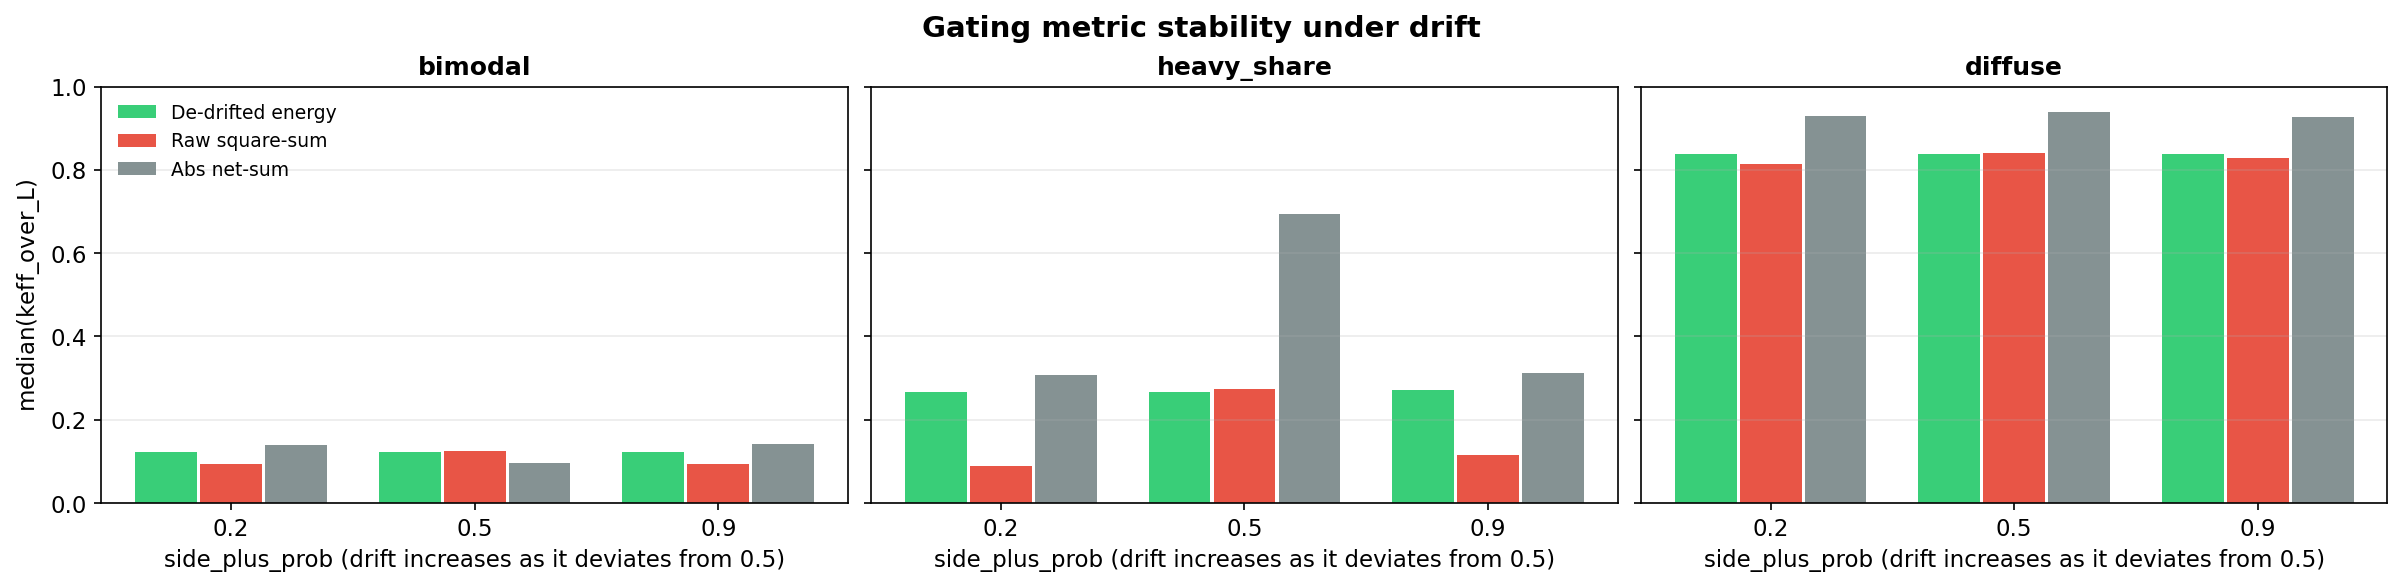
\includegraphics[width=0.9\textwidth]{figures/fig_exp03v2_gating_keff_over_L_vs_drift.png}
\caption{Drift stability of gating under high-pressure configurations ($B \in \{100, 500\}$). The $K_{\mathrm{eff}}/L$ of de-drifted energy remains nearly constant within each workload as drift varies; the first moment exhibits anomalous inflation at $q{=}0.5$.}
\label{fig:c2-4}
\end{figure*}

The main text (\S\ref{sec:eval-dedrift}) confirmed that $K_{\mathrm{eff}}/L$ computed from de-drifted energy remains stable under drift in the base configuration ($B{=}10$). Table~\ref{tab:c2-5} and Figure~\ref{fig:c2-4} extend this validation to high-pressure configurations ($B{=}500$).
The $K_{\mathrm{eff}}/L$ of de-drifted energy stays within the narrow band of $0.426$--$0.430$ across three drift conditions, despite the absolute value increasing from $\sim 0.016$ ($B{=}10$, Table~\ref{tab:c2-5}) to $\sim 0.43$ due to the larger $B$.
As a control, the first moment (\texttt{abs\_net\_sum}) at $q{=}0.5$ is inflated to $0.745$.


\subsection{Insensitivity to De-drifting}

\begin{figure*}[!htbp]
\centering
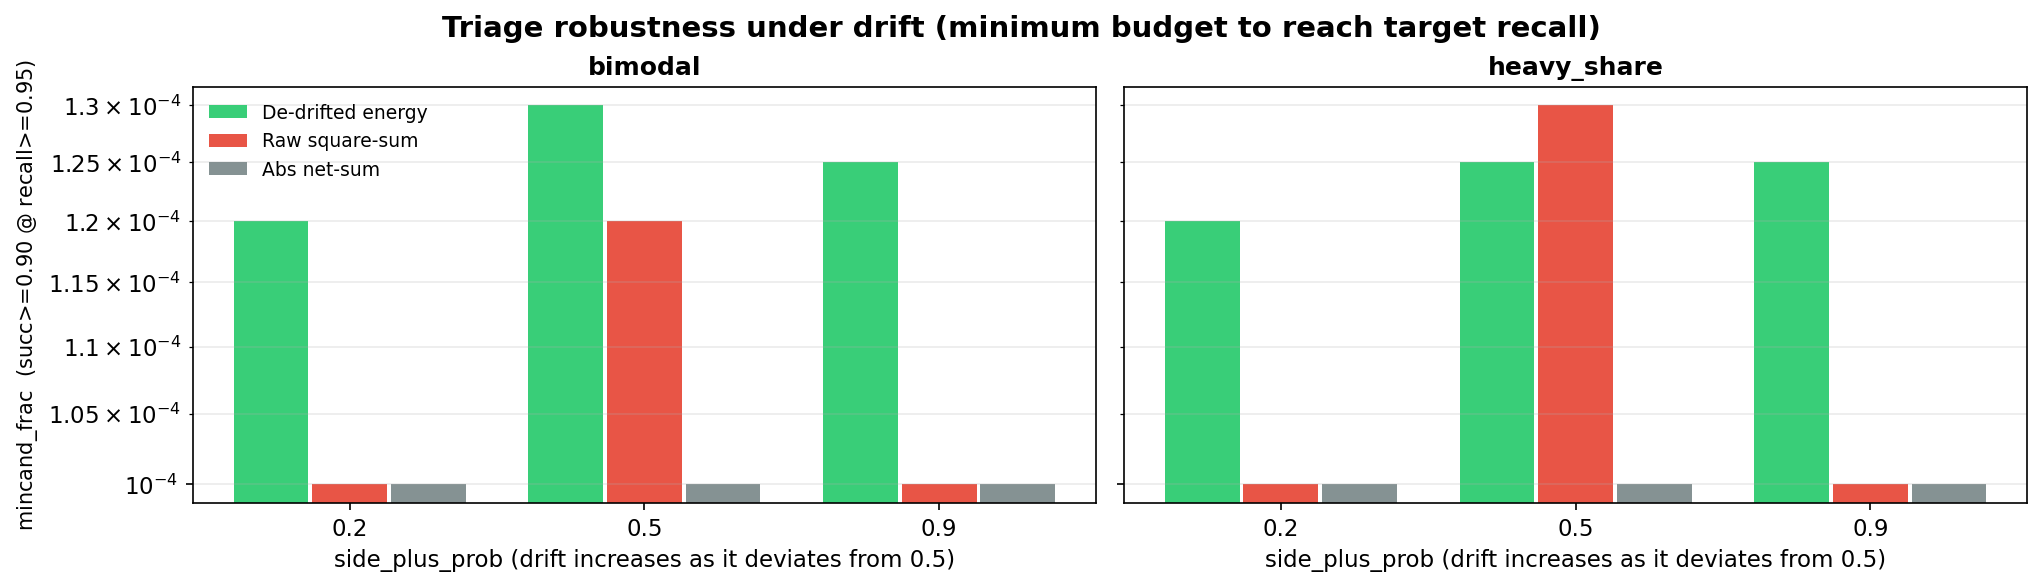
\includegraphics[width=0.8\textwidth]{figures/fig_exp03v2_triage_mincand_vs_drift.png}
\caption{Triage under drift sweep. The figure plots the minimum \texttt{cand\_frac} required by the three statistics as drift varies.}
\label{fig:c2-a1}
\end{figure*}

The preceding sections established the necessity of de-drifting for sizing and gating. A natural follow-up question is whether triage similarly requires de-drifting. Figure~\ref{fig:c2-a1} compares the minimum \texttt{cand\_frac} required by the three statistics on the same drift sweep grid, using the operating point framework (\S\ref{sec:eval-operating}).
Within the tested range, all three statistics exhibit comparable variation with drift, and no additional failure mode induced by drift is observed in the triage dimension.

Accordingly, we use the same de-drifted energy for sizing, gating, and triage. This choice introduces no additional probe overhead and incurs no observable penalty on triage metrics.




